\documentclass[5p,times,sort&compress]{elsarticle}

\usepackage[utf8]{inputenc}
\usepackage{amsmath}
\usepackage{amssymb}
\usepackage{amsopn}
\usepackage{mathtools}
\usepackage{bm}
\usepackage[table]{xcolor}
\usepackage{textcomp}
\usepackage{float}
\usepackage{placeins}
\usepackage{gensymb}
\usepackage{dblfloatfix}
\usepackage{chemformula}
\usepackage{siunitx}
\sisetup{detect-all}
\DeclareSIUnit{\atpercent}{at.\%}
\DeclareSIUnit{\wtpercent}{wt.\%}
\DeclareSIUnit{\gramforce}{gf}
\DeclareSIUnit{\angstrom}{\protect \text {Å}}
\usepackage{graphicx}
\graphicspath{{../figures/}}
\usepackage[table,dvipsnames]{xcolor}
\definecolor{Gray}{gray}{0.9}
\definecolor{dkgreen}{rgb}{0,0.6,0}
\definecolor{gray}{rgb}{0.5,0.5,0.5}
\definecolor{mauve}{rgb}{0.58,0,0.82}
\usepackage{booktabs}
\usepackage{multirow}
\usepackage{array}
\usepackage{dblfloatfix}
\usepackage{tabularx}
\usepackage{colortbl}
\usepackage{lscape}
%\usepackage{stfloats}
\usepackage{makecell}
 \usepackage{afterpage}
\usepackage{nicematrix}
\usepackage{float}
\usepackage{subcaption}
\usepackage{tikz}
\usetikzlibrary{positioning}
\usepackage{cuted}
\usepackage{hyperref}
\setlength{\abovedisplayskip}{12pt}
\setlength{\belowdisplayskip}{12pt}
\setlength{\abovedisplayshortskip}{12pt}
\setlength{\belowdisplayshortskip}{12pt}
\hypersetup{
    hidelinks,
    breaklinks=true,
    colorlinks=false,
    linkcolor=black,
    citecolor=black,
    urlcolor=black
}
\usepackage{xr-hyper}
\usepackage{listings}
\lstset{frame=tb,
  language=Python,
  aboveskip=3mm,
  belowskip=3mm,
  showstringspaces=false,
  columns=flexible,
  basicstyle={\small\ttfamily},
  numbers=none,
  numberstyle=\tiny\color{gray},
  keywordstyle=\color{blue},
  commentstyle=\color{dkgreen},
  stringstyle=\color{mauve},
  breaklines=true,
  breakatwhitespace=true,
  tabsize=3
}
\usepackage{cleveref}
\usepackage{placeins}
\usepackage{dblfloatfix}

\usepackage{lineno}
%\linenumbers  % Uncomment this for line-numbers

%\journal{Acta Materialia}

\makeatletter
\def\ps@pprintTitle{%
 \let\@oddhead\@empty
 \let\@evenhead\@empty
 \def\@oddfoot{}%
 \let\@evenfoot\@oddfoot}
\makeatother

\newcommand{\argmax}{\operatornamewithlimits{argmax}}
\newcommand{\etal}{\textit{et al.~}}

\newcommand{\dogu}[1]{\textcolor{red}{\textit{Doğu}: #1}}
\newcommand{\brent}[1]{\textcolor{blue}{\textit{Brent}: #1}}
\newcommand{\samuel}[1]{\textcolor{green}{\textit{Samuel}: #1}}

% \renewcommand{\dogu}{}

\begin{document}

\sloppy

\begin{frontmatter}

%\title{Constraint-First Screening of Low-Activation Refractory Alloys via Linear Programming}

%\title{Design of Terminal Compositions for Joinable/FGM-able Alloy System for Fusion Materials}



%\title{Computational Design of a Doubly-Monotonic Functionally Graded Refractory Alloy for the Fusion First Wall}

%\title{Computational Design of a Doubly-Monotonic Functionally Graded Refractory Alloy for Fusion First Wall Applications}

%\title{Computational Design of a Functionally Graded Refractory Alloy with Monotonic Thermal Expansion and Solidus for Fusion First Wall Applications}

%\title{Computational Design of a Compositionally Graded Refractory Alloy with Monotonic Thermal Expansion and Solidus for the Fusion First Wall}

%\title{Computational Design of a Reduced-Activation Compositionally Graded Refractory Alloy for the Fusion First Wall}

\title{Computational Design of a Reduced-Activation Compositionally Graded Refractory Alloy for Fusion Applications}

\author[1]{Samuel Ifada\texorpdfstring{\corref{cor1}}{}}
\author[1]{Brent Vela}
\author[1]{James Hanagan}
\author[1]{Do\u{g}uhan Sar\i{}t\"urk}
\author[1,2,3]{Raymundo Arr\'oyave}

\affiliation[1]{organization={Department of Materials Science and Engineering, Texas A\&M University},
                city={College Station},
                postcode={77843}, 
                state={TX},
                country={USA}}

\affiliation[2]{organization={J. Mike Walker '66 Department of Mechanical Engineering, Texas A\&M University},
                city={College Station},
                postcode={77843}, 
                state={TX},
                country={USA}}

\affiliation[3]{organization={Wm Michael Barnes '64 Department of Industrial and Systems Engineering, Texas A\&M University},
                city={College Station},
                postcode={77843}, 
                state={TX},
                country={USA}}


%\begin{abstract}
%In alloy design, constraint-driven screening is traditionally performed by a generate-and-filter workflow, in which every candidate composition on a discrete grid is evaluated with a response model and filtered against performance thresholds. This incurs a cost proportional to the full composition grid, even when only a small fraction of candidates satisfy the constraints. Here we present an alternative framework that reformulates screening as a linear-programming (LP) feasibility problem whenever the response model is linear in alloy composition. Under this formulation, the compositions satisfying all screening criteria form a convex polytope on the atomic-fraction simplex, and the feasible compositions are obtained by enumerating the grid points within this polytope directly, rather than by explicit per-composition response evaluation. We demonstrate the approach using FLARE, a linear-in-composition activation model, to identify candidate plasma-facing and structural alloys for a two-material fusion first wall, screening an eleven-element refractory system against activation limits referenced to tungsten and EUROFER97. The LP-defined feasible set reproduces that of the conventional FLARE generate-and-filter workflow exactly, recovering the identical compositions and activation responses while replacing the evaluation of all \(\sim\!3\times10^{7}\) grid candidates with a direct analytical representation of the feasible space. More broadly, the constraint-first LP framework applies to any alloy-screening workflow governed by response models that are linear in composition.
%\end{abstract}

%\begin{keyword}
%linear programming \sep constraint-first screening \sep feasible composition polytope \sep high-throughput alloy design \sep FLARE \sep low-activation refractory alloys
%\end{keyword}

\begin{abstract}

The first wall of a fusion reactor combines a tungsten-rich plasma-facing material with a load-bearing structural alloy, and the joint between them is limited by thermal-expansion mismatch and by the formation of brittle W--Fe intermetallic phases. Compositionally graded alloys (CGAs) can spread this mismatch over many layers, but the intermediate compositions must also remain single-phase, reduced in activation, and strong, a combination that is difficult to identify by hand in a multicomponent composition space. In this work, a CGA for the first wall is designed computationally in the eleven-element Cr-Fe-Hf-Mo-Nb-Re-Ta-Ti-V-W-Zr system. Reduced-activation compositions are obtained directly by linear programming on the composition-linear FLARE activation model, screened by CALPHAD for single-phase BCC stability and thermal conductivity, and classified as plasma-facing or structural materials by solidus, Pugh ratio, and EUROFER97-level yield strength. The gradient path between the two terminal alloys is then planned on a composition graph using the lack-of-monotonicity cost function of Kirk et al., with the coefficient of thermal expansion (CTE) required never to decrease and the solidus never to increase from the plasma-facing side to the structural side. With both requirements imposed as hard constraints, the cost reduces to path length, and the optimal path is found exactly by Dijkstra's algorithm. The resulting path joins W$_{90}$V$_{5}$Re$_{5}$ to W$_{15}$V$_{75}$Ti$_{10}$ in sixteen 5~at.\% steps, the minimum possible for these terminals. Along it, the linear CTE at 600~$^{\circ}$C rises from 5.03 to 9.28$\times10^{-6}$~K$^{-1}$ in increments of at most 0.28$\times10^{-6}$~K$^{-1}$, the solidus falls from 3449 to 2262~K, and every layer is single-phase BCC, reduced in activation, and at least as strong as EUROFER97 at 600 and 650~$^{\circ}$C. The approach applies generally to graded-alloy design problems governed by composition-linear screening models and monotonic property requirements.
\end{abstract}

\begin{keyword}
compositionally graded alloys \sep fusion first wall \sep
reduced-activation refractory alloys \sep linear programming \sep
path planning \sep property monotonicity
\end{keyword}

\end{frontmatter}

\section{Introduction}

The first wall of a fusion reactor is a two-material system. A plasma-facing
material meets the plasma, withstanding extreme heat flux, particle bombardment,
and neutron irradiation, while a structural alloy behind it carries the mechanical
load. Tungsten is the leading plasma-facing material owing to its high melting
point, low sputtering yield, and good thermal conductivity, but it is brittle and
unsuited to a load-bearing role~\cite{tungstenPFMreview2023}. Reduced-activation
ferritic-martensitic (RAFM) steels such as EUROFER97 serve as the structural
material, with favorable activation but limited high-temperature
capability~\cite{lindau2005eurofer,RAFMreview2017}. Both must also resist
irradiation damage and remain acceptably activated through operation and
decommissioning~\cite{zinkle2000operating,bloom2007critical}. As no single material
satisfies the surface and structural requirements simultaneously, the first wall
must be built from a plasma-facing material and a structural material joined into
one component.

Joining these materials is a central difficulty. Tungsten and steel differ
markedly in thermal expansion, with coefficients of roughly \(4.4\) and
\(12.7 \times 10^{-6}\)~K\(^{-1}\), so an abrupt joint concentrates large thermal
stresses, and direct tungsten--iron contact forms brittle intermetallics,
principally Fe\(_2\)W and Fe\(_7\)W\(_6\), that embrittle the
joint~\cite{fgmWsteelCGS2022,karim2024wire}. Functionally graded materials (FGMs),
in which composition or structure varies with position, offer a potential solution.
A compositionally graded alloy (CGA), a subset of FGMs in which the alloy
composition varies gradually from one terminal alloy to another, can spread the
expansion mismatch over a graded region rather than a single
boundary~\cite{fgmWEurofer2015}. Such gradients are now practically realizable, as
additive manufacturing (AM) processes such as directed energy deposition can vary
the feed composition layer by layer~\cite{karim2024wire}.

Despite these advances in manufacturing capability, grading alone does not avoid
the intermetallics, since iron and tungsten still meet across the gradient. One
remedy is to keep the transition a single body-centered cubic (BCC) solid solution
at every layer, so that the gradient never enters the composition ranges where the
brittle phases are stable~\cite{fgmWsteelInterlayerBCC2023}. This choice changes
the structural terminal itself. Rather than grading toward a steel, the gradient can
terminate in a vanadium-rich structural alloy that is reduced in activation and
reachable from tungsten through a continuous BCC path, so that iron and tungsten
never meet along the transition. Existing realizations, however, rely on a few
interlayers selected by hand, one composition at a
time~\cite{fgmWsteelInterlayerBCC2023}. Identifying such a path by inspection is a
fundamentally limited approach, since the constraints interact across a
composition space far too large to visualize.

The constraints are also numerous. The plasma-facing side requires high-temperature
capability and the structural side requires ductility, while reduced activation, a
stable single-phase structure, adequate thermal conductivity, and sufficient
strength must be met by both terminals and every intermediate layer alike.
Multicomponent refractory alloys offer wide freedom to balance these
demands~\cite{HEAnuclear2021,Senkov2010}, and high-throughput screening that
combines CALculation of PHAse Diagrams (CALPHAD) thermodynamics with physics-based
strength and ductility models has proven effective in reducing such spaces to
actionable candidate sets~\cite{vela2023data,HTcalphad2022}. Among the criteria,
neutron-induced activation is especially consequential, since transmutation governs
decay heat, dose rates, maintenance, and waste burden~\cite{RAFMreview2017}. The
FLARE model makes this criterion tractable by expressing the activation response of
any alloy as a composition-weighted sum of precomputed elemental
responses~\cite{Marquez2026FLARE}. Because these responses are linear in
composition, the compositions satisfying all activation limits form a convex
polytope that can be obtained directly by linear programming, without evaluating
the candidates one by one.

Computational path planning offers a systematic alternative to hand-selected
interlayers. Kirk et al.\ adapted motion-planning algorithms from robotics to plan
gradient paths through high-dimensional composition spaces while avoiding regions
of undesirable phases~\cite{kirk2018gradient}, an approach subsequently
demonstrated in additively manufactured gradients~\cite{eliseeva2019fgm}. The
framework was later extended to paths with monotonic property profiles, using a
lack-of-monotonicity cost function, on the argument that a monotonic gradient can
be transformed into nearly any spatial profile on the part by controlling the
deposition rate~\cite{kirk2021monotonic}. This cost function has since been used to
design and print a gradient that is monotonic in stacking fault
energy~\cite{hanagan2025sfe}, and monotonic property profiles have also been
imposed in graded deposition, where a liquidus that falls along the build prevents
the remelting of previously deposited layers~\cite{glerum2026ss316tzm}. More
recently, the composition space has been represented as a graph of feasible
compositions, enabling the design of multi-terminal graded
structures~\cite{multiterminalCGA2024} and the identification of connected feasible
regions for CGA design~\cite{obrist2026graph}. These methods, however, have treated
monotonicity in a single property at a time. The first wall requires two at once:
a coefficient of thermal expansion (CTE) that never decreases, so that the
expansion mismatch at every interface acts in the same direction, and a solidus
that never increases, so that no layer melts at a lower temperature than a layer
behind it, which faces a lower temperature in service. Both must hold along a path
whose every composition also satisfies activation, phase-stability, conductivity,
and strength constraints.

In this work, a CGA for the fusion first wall is designed in the eleven-element
refractory system \ch{Cr-Fe-Hf-Mo-Nb-Re-Ta-Ti-V-W-Zr}. Activation screening by
linear programming, referenced to tungsten and EUROFER97, defines the feasible
composition space. CALPHAD calculations reduce this space to a connected,
single-phase BCC design region, whose compositions are classified as plasma-facing
or structural materials by solidus, Pugh ratio, and EUROFER97-level yield strength.
The gradient path between the two terminal alloys is then planned on the
composition graph with the cost function of Kirk et al.~\cite{kirk2021monotonic},
with monotonicity in both CTE and solidus imposed as hard constraints. Under these
constraints the cost reduces to path length, and the optimal path is found exactly
by Dijkstra's algorithm, with no penalty weight to tune. The approach improves upon
previous work by enabling monotonicity in more than one property at once while
every layer remains reduced in activation, single-phase, and at least as strong as
EUROFER97.

The remainder of this paper is organized as follows. First, the activation
screening, property calculations, and gradient path design problem are described in
Section~\ref{sec:methods}. The resulting feasible space, design region, terminal
alloys, and gradient path are then presented and discussed in
Section~\ref{sec:results}. Finally, conclusions and future work are given in
Section~\ref{sec:conclusion}. The overall workflow is summarized in
Fig.~\ref{fig:overview}.

\begin{figure*}[!t]
  \centering
  \includegraphics[width=0.9\textwidth]{figures/FGM-SCHEMATIC.png}
 \caption{Overview of the design workflow: activation screening by linear
programming, property filtering and classification of the feasible composition
space, selection of the plasma-facing and structural terminal alloys, and gradient
path design with monotonic CTE and solidus.}
  \label{fig:overview}
\end{figure*}

\section{Methods}
\subsection{Activation Screening by Linear Programming}
\label{sec:feasible-space}

The low-activation feasible space is defined over the eleven-element
\ch{Cr-Fe-Hf-Mo-Nb-Re-Ta-Ti-V-W-Zr} system, sampled on a \(5\)~at.\% grid, using
the \emph{FLARE} activation model~\cite{Marquez2026FLARE} together with linear programming.
\emph{FLARE} is a reduced-order model that estimates the neutron-activation
response of an alloy, gas generation, displacement damage, decay heat, and contact
dose rate, as a composition-weighted sum of precomputed elemental contributions,
providing a quantitative basis for assessing irradiation-induced phenomena across
the design space.

The responses are evaluated under the irradiation conditions summarized in
\Cref{tab:ind_variables}, a two-year irradiation time with decay times of one
second, one month, and 100 years, corresponding to the immediate post-irradiation,
maintenance, and long-term waste management scenarios. Under these conditions, the
responses of pure W and EUROFER97 serve as reference baselines for plasma-facing
and structural materials, respectively, and a composition is retained if each of
its responses stays within a deviation factor of \(\phi=10\) of the corresponding
baseline value.

\begin{table}[H]
\centering
\caption{Summary of irradiation condition inputs used in the \emph{FLARE} model to
evaluate activation responses for candidate alloys under first-wall neutron
environments.}
\label{tab:ind_variables}
\begin{tabularx}{\columnwidth}{lX}
\toprule
\multicolumn{2}{c}{\textbf{Independent Variables}} \\
\midrule
First Wall Average Neutron Flux & \(8\times10^{13}~\mathrm{n/cm^2 s}\) \\
Irradiation Time               & 2 years \\
Decay Time                     & 1 second \& 1 month \& 100 years \\
\bottomrule
\end{tabularx}
\end{table}

The conventional way to apply these baselines is to generate every composition,
evaluate its responses, and discard those that fall outside the limits. For a
\(5\)~at.\% grid this requires testing on the order of \(10^{7}\) compositions one
by one, which is slow and scales poorly as elements or resolution are added. We
avoid this entirely by using the structure of the screening problem itself, since
the FLARE responses are linear in the alloy composition
\(\mathbf{x}=(x_1,\dots,x_N)\), directly for the atomic-fraction-averaged
displacement damage and, for the mass-weighted responses, once each criterion
is multiplied through by their common alloy-mass denominator. Linearity is what makes the shortcut
possible, since when a response varies linearly with composition, the boundary at which it crosses
a baseline limit is a flat surface in composition space, so each limit simply
divides the space into an allowed and a disallowed side rather than having to be
tested point by point. Each baseline limit is therefore a linear inequality in
\(\mathbf{x}\), and stacking all of them, with the simplex condition
\(\sum_i x_i = 1\) and the bounds \(0 \le x_i \le 1\), gives a single linear
system \(\mathbf{G}\mathbf{x} \le \mathbf{h}\). The compositions satisfying
every limit are exactly those lying inside the region enclosed by these surfaces, a
convex polytope

\begin{equation}
P=\{\mathbf{x}\in\Delta : \mathbf{G}\mathbf{x}\le\mathbf{h}\}.
\label{eq:polytope}
\end{equation}

The feasible region is thus obtained directly as \(P\) by linear programming, and
the \(5\)~at.\% grid compositions inside it are enumerated without evaluating the
infeasible majority of the grid. This is substantially faster than
generate-and-filter and, importantly, it is not specific to FLARE, as the same
construction applies to any screening model whose responses are linear in
composition, FLARE being one such model. The resulting low-activation feasible
space is the starting point for the property evaluation and graded-path design that
follow.

\subsection{Property Calculations}
\label{sec:feasible-space-props}

Following activation screening, the surviving compositions were characterized by
high-throughput calculations of the properties on which the design depends. Because
direct experimental characterization is impractical for the number of candidates
considered, physically motivated models were used as first-order estimates: the
Maresca--Curtin model for yield strength, the Pugh ratio for intrinsic ductility,
and CALPHAD for phase stability, melting behavior, and thermophysical properties.

Yield strength was estimated with the Maresca--Curtin (MC) model for
body-centered cubic random solid solutions~\cite{maresca2020mechanistic},
following the methodology previously applied to the screening of refractory
multi-principal-element alloys~\cite{vela2023data}. The model relates strength to
the energetics of thermally activated dislocation glide, with the
temperature-dependent yield strength given by
\begin{equation}
\tau_y(T,\dot{\varepsilon})
= \tau_{y0}
\exp\!\left[
-\frac{1}{0.55}
\left(
\frac{kT}{\Delta E_b}
\ln\!\left(\frac{\dot{\varepsilon}_0}{\dot{\varepsilon}}\right)
\right)^{0.91}
\right],
\label{eq:yield_stress}
\end{equation}
where $\tau_{y0}$ is the athermal yield strength, $\Delta E_b$ is the
activation barrier for dislocation glide, $T$ is the absolute temperature,
$\dot{\varepsilon}$ is the applied strain rate, $\dot{\varepsilon}_0$ is the
reference strain rate, and $k$ is Boltzmann's constant, with the tensile
yield strength obtained through the appropriate Taylor-factor conversion. The
physical inputs, including atomic volumes, elastic constants ($C_{11}$, $C_{12}$,
and $C_{44}$), shear moduli, and Poisson ratios, were assembled from literature
data and combined by the rule of mixtures. Yield strengths were evaluated at 600
and $650^{\circ}\mathrm{C}$, the service temperatures considered for the
plasma-facing and structural sides of the wall, at a strain rate of
$10^{-3}\,\mathrm{s}^{-1}$, and are used as design criteria in
Section~\ref{sec:joinable}.

Intrinsic ductility was assessed with the Pugh ratio \(B/G\), the ratio of bulk to
shear modulus, in the modern convention in which larger values indicate greater
ductility~\cite{pugh1954,singh2023ductility}. The elemental Poisson ratios
\(\nu_i\) were combined by the rule of mixtures, \(\bar{\nu}=\sum_i x_i \nu_i\),
where $x_i$ is the atomic fraction of element $i$, and through the isotropic
relations \(E=3B(1-2\nu)\) and \(G=E/2(1+\nu)\) the descriptor reduces to
\begin{equation}
\frac{B}{G}=\frac{2\,(1+\bar{\nu})}{3\,(1-2\bar{\nu})}.
\label{eq:pugh}
\end{equation}
A composition is considered intrinsically ductile when \(B/G \ge 2.6\), a stricter
cutoff than the conventional \(B/G > 1.75\) criterion~\cite{singh2023ductility}.
As a rule-of-mixtures prior, this descriptor serves as a screening-level estimate.

Phase stability, melting behavior, and thermophysical properties were obtained with
the CALPHAD (CALculation of PHAse Diagrams) method, in which the Gibbs free energy
of every candidate phase is described by parametric models assessed from
experimental and first-principles data and extrapolated to multicomponent
alloys~\cite{li2023calphad,conway2022thermodynamic}. Calculations were performed
with Thermo-Calc's TC-Python API and the TCHEA6 database, assessed for
high-entropy and refractory multi-principal-element systems. Equilibrium phase
fractions, including the BCC solid solution and competing intermetallic phases such
as sigma, Laves, mu, and chi, were computed at 500, 600, and
$650^{\circ}\mathrm{C}$. The solidus temperature \(T_s\) was obtained with the
Liquidus and Solidus Temperature property model, and the thermal conductivity at
$25^{\circ}\mathrm{C}$ and the linear coefficient of thermal expansion (CTE)
\(\alpha\) at 600 and $650^{\circ}\mathrm{C}$ with the Equilibrium with Freeze-in
temperature property model.

\subsection{Graded-Path Design}
\label{sec:joinable}

The activation-feasible compositions were first screened for single-phase BCC
stability and heat removal, retaining a composition only if
\begin{equation}
f_{\mathrm{BCC}}(T) \ge 0.98 \quad (T = 500,\ 600,\ 650\ ^{\circ}\mathrm{C}),
\qquad \kappa_{25\,^{\circ}\mathrm{C}} > 16~\mathrm{W\,m^{-1}\,K^{-1}},
\label{eq:filters}
\end{equation}
where \(f_{\mathrm{BCC}}\) is the BCC phase fraction and \(\kappa\) the thermal
conductivity. The surviving compositions were organized into a simplex-lattice
graph~\cite{nimplex}, in which two compositions \(u\) and \(v\) are neighbors when
they differ by a single grid step,
\(\mathbf{x}_v-\mathbf{x}_u = 0.05\,(\mathbf{e}_b-\mathbf{e}_a)\), one element
decreased and another increased by one increment. Graph representations of the
design space have likewise been used for the design of compositionally graded
structures~\cite{multiterminalCGA2024}. Because the screens remove compositions
unevenly, the graph separates into connected subgraphs, and the largest is carried
forward as the design region since it offers the widest contiguous space for a
graded transition~\cite{obrist2026graph}.

Each composition of the design region is classified by the property the two sides
of the first wall require. A composition is a plasma-facing candidate,
Material~A, or a structural candidate, Material~B, when
\begin{equation}
\text{A:}\ \ T_s > 2200~^{\circ}\mathrm{C}\ \text{and}\ \sigma_y^{600} \ge 300~\mathrm{MPa},
\qquad
\text{B:}\ \ B/G \ge 2.6\ \text{and}\ \sigma_y^{650} \ge 250~\mathrm{MPa},
\label{eq:classes}
\end{equation}
where \(\sigma_y^{T}\) is the yield strength at \(T\)~\(^{\circ}\)C. The strength
limits are set at the level of the reference structural steel
EUROFER97~\cite{lindau2005eurofer}, so that every candidate is at least as strong as
the steel it would replace at the service temperatures.
Compositions satisfying both definitions form Material~AB, and those satisfying
neither are classified as Intermediate. The two ends of the gradient are chosen by
the function of each side of the wall, as in previous gradient design
studies~\cite{kirk2021monotonic}: the plasma-facing (PFM) end is the
highest-solidus composition of Material~A or AB, and the structural end the
highest-Pugh-ratio composition of Material~B or AB,
\begin{equation}
v_{\mathrm{PFM}} = \arg\max_{v \in A \cup AB} T_s(v), \qquad
v_{\mathrm{str}} = \arg\max_{v \in B \cup AB} (B/G)(v).
\label{eq:ends}
\end{equation}

A graded path \(P=(v_0,v_1,\dots,v_L)\), with \(v_0=v_{\mathrm{PFM}}\) and
\(v_L=v_{\mathrm{str}}\), is a sequence of neighboring compositions, each step
corresponding to one deposited layer. Every layer must be a design material that is
at least as strong as EUROFER97 at both service temperatures and a multicomponent
alloy, so the admissible compositions are
\begin{equation}
\mathcal{V} = \{\, v \in A \cup B \cup AB :\ \sigma_y^{600}(v) \ge 300~\mathrm{MPa},\
\sigma_y^{650}(v) \ge 250~\mathrm{MPa},\ N_{\mathrm{el}}(v) \ge 3 \,\},
\label{eq:admissible}
\end{equation}
where \(N_{\mathrm{el}}\) is the number of constituent elements. Two monotonicity
constraints are imposed on every step \(u \to v\),
\begin{equation}
\alpha_T(v) \ge \alpha_T(u) \quad (T = 600,\ 650\ ^{\circ}\mathrm{C}),
\qquad T_s(v) \le T_s(u).
\label{eq:monotone}
\end{equation}
A monotonic CTE keeps the thermal-expansion mismatch at every interface in the same
direction, from the low-expansion plasma-facing alloy to the higher-expansion
structural alloy, so that no interlayer reverses the strain gradient across the
wall~\cite{kirk2021monotonic}. A monotonic solidus follows the temperature profile
of the wall, which falls from the plasma-facing surface toward the coolant, so that
no layer has a lower melting point than a layer behind it, in the same way that a
monotonic liquidus prevents remelting of previously deposited layers during graded
deposition~\cite{glerum2026ss316tzm}. These constraints are imposed on the graph
itself: each undirected edge is expanded into its two directed steps, and a step is
kept only if both compositions belong to \(\mathcal{V}\) and it satisfies
\Cref{eq:monotone}.

The path cost follows Kirk et al.~\cite{kirk2021monotonic}, a monotonicity
penalty plus a small path-length weight,
\begin{equation}
c(P) = \mathrm{LOI}(P) + w\,l(P), \qquad w \ll 1,
\label{eq:cost}
\end{equation}
where the loss of invariance, LOI, is the total change of the constrained
properties against their required direction and \(l\) is the path length in
composition space,
\begin{equation}
\mathrm{LOI}(P)=\sum_{k=1}^{L}\Big[\sum_{T}\max\!\big(\alpha_T(v_{k-1})-\alpha_T(v_k),0\big)
+\max\!\big(T_s(v_k)-T_s(v_{k-1}),0\big)\Big],
\qquad
l(P)=\sum_{k=1}^{L}\lVert \mathbf{x}_{v_k}-\mathbf{x}_{v_{k-1}}\rVert_2 .
\label{eq:loi}
\end{equation}
Because the monotonicity constraints are imposed as hard rules, \(\mathrm{LOI}=0\) on
every admissible path, and since every step is a single 5~at.\% exchange,
\(l = 0.05\sqrt{2}\,L\). The cost therefore reduces to the number of steps, and the
design path is the shortest monotonic path,
\begin{equation}
P^{*} = \arg\min_{P}\, L(P),
\label{eq:shortest}
\end{equation}
which is found exactly by Dijkstra's algorithm~\cite{dijkstra1959note} with unit
step weights on the directed graph of admissible monotonic steps. Because every
composition property is computed once and stored with the graph, the search
returns the optimal path exactly rather than approximately, in contrast to the
sampling-based planners used previously~\cite{kirk2021monotonic,kirk2018gradient}.
Several paths can share the minimum length; they are equally optimal under this
cost, and the algorithm returns one of them deterministically. The returned path is
verified step by step against \Cref{eq:admissible,eq:monotone}.

\begin{figure*}[!t]
  \centering
  \includegraphics[width=0.75\textwidth]{figures/LP-FLARE-polytope-5at-10x.pdf}
  \caption{Activation-feasible compositions from the LP screen, projected onto the
eleven-element composition simplex. The left panel shows the \(10\times\)W
feasible region, and the right panel the \(10\times\)EUROFER97 region, with feasible
compositions as points and the projected vertex hull outlined.}
  \label{fig:polytope}
\end{figure*}

\section{Results and Discussion}
\label{sec:results}

\subsection{Activation-Feasible Space}
\label{subsec:feasible}
The \(5\)~at.\% grid of the eleven-element system contains \(30{,}045{,}015\)
compositions. The LP construction identifies \(210\) of them as feasible under the
\(10\times\)W reference and \(61{,}297\) under the \(10\times\)EUROFER97 reference
(Fig.~\ref{fig:polytope}), the two sets corresponding to the plasma-facing and
structural sides of the wall. The difference of more than two orders of magnitude
reflects the lower activation of pure W, for which ten times the baseline is the
tighter bound. Although all eleven elements were free to vary, Ta, Nb, Mo, and Hf do
not occur in either set: they are excluded by activation alone, before any property
is considered. Every composition retained here, and therefore every layer of the
final gradient, stays within a factor of ten of its reference material for all
activation responses under the conditions of Table~\ref{tab:ind_variables}.

The LP construction returned exactly the compositions found by brute-force FLARE
evaluation of the full grid, with every response agreeing to numerical precision,
at a fraction of the cost (Table~\ref{tab:benchmark}). Brute force evaluates all
\(30{,}045{,}015\) grid compositions, whereas the LP approach evaluates only those
inside the polytope, reducing the wall-clock time from
\textcolor{red}{[\,\(t_{\mathrm{BF}}\)\,]} to \textcolor{red}{[\,\(t_{\mathrm{LP}}\)\,]}
and the peak memory from \textcolor{red}{[\,\(m_{\mathrm{BF}}\)\,]} to
\textcolor{red}{[\,\(m_{\mathrm{LP}}\)\,]}. The brute-force cost grows with the number
of grid points, which increases combinatorially with the number of elements and the
grid resolution, while the LP cost grows with the size of the feasible set, so the
advantage widens as the design space is refined.

\begin{table}[H]
\centering
\caption{Cost of identifying the activation-feasible compositions by brute-force
evaluation and by the LP construction, for both references. Hardware and software
are given in Section~\ref{sec:feasible-space}.}
\label{tab:benchmark}
\begin{tabularx}{\columnwidth}{lXX}
\toprule
 & Brute force & LP \\
\midrule
Compositions evaluated       & \(30{,}045{,}015\) & \textcolor{red}{[\,\,]} \\
Feasible, \(10\times\)W        & \(210\)            & \(210\) \\
Feasible, \(10\times\)EUROFER97 & \(61{,}297\)      & \(61{,}297\) \\
Wall-clock time              & \textcolor{red}{[\,\,]} & \textcolor{red}{[\,\,]} \\
CPU cores used               & \textcolor{red}{[\,\,]} & \textcolor{red}{[\,\,]} \\
Peak memory                  & \textcolor{red}{[\,\,]} & \textcolor{red}{[\,\,]} \\
Speed-up                     & \(1\times\)        & \textcolor{red}{[\,\,]} \\
\bottomrule
\end{tabularx}
\end{table}


\subsection{Phase Stability, Thermal Conductivity, and the Design Region}
\label{subsec:subgraphs}

Merging the two activation-feasible sets, in which \(204\) compositions are feasible
under both references, gives \(61{,}303\) unique compositions. Of these, \(700\)
(\(1.1\%\)) satisfy the phase-stability and conductivity criteria of
\Cref{eq:filters}. Phase stability is the decisive filter: \(50{,}365\) compositions
conduct heat adequately, but only \(706\) remain single-phase BCC at all three
temperatures. The reduced-activation space is therefore dominated by compositions
that would form intermetallics in service, and a gradient designed without a phase
constraint would almost certainly pass through them.

On the composition graph, the \(700\) compositions form three disconnected subgraphs
(Fig.~\ref{fig:clusters}). Subgraph~1 holds \(686\) compositions, \(98\%\) of the
total, extending from the tungsten-rich corner through the vanadium- and
titanium-rich region toward chromium. Subgraphs~2 and~3 are islands of eight and six
compositions, near the Fe corner and in the interior of the simplex, that satisfy
every screen yet cannot be reached from Subgraph~1 without passing through a
composition that fails one. Subgraph~1 is the only region in which a gradient can be
built from feasible layers alone, and it is the design region.

\begin{figure}[H]
  \centering
  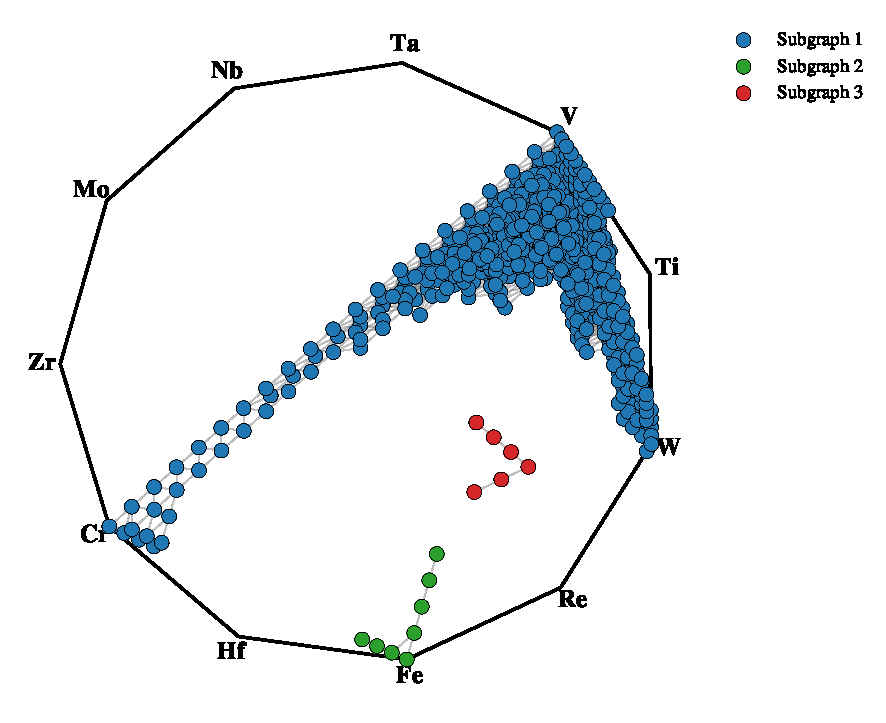
\includegraphics[width=0.75\linewidth]{figures/fig1_subgraphs.pdf}
  \caption{Connected subgraphs of the \(700\) compositions that pass the
  activation, single-phase BCC, and thermal-conductivity screens, projected onto
  the eleven-element composition space, with each element at a vertex. Circled
  numbers identify the subgraphs: Subgraph~1 (blue, \(686\) compositions) is the
  design region, and Subgraphs~2 (green) and~3 (red) are isolated islands of eight
  and six compositions.}
  \label{fig:clusters}
\end{figure}


\subsection{Plasma-Facing and Structural Materials}
\label{subsec:classification}

Classifying the design region by the two sides of the wall (\Cref{eq:classes})
gives \(139\) plasma-facing compositions (Material~A), \(169\) structural
compositions (Material~B), and \(18\) that qualify for both (Material~AB); the
remaining \(360\) are Intermediate (Fig.~\ref{fig:categories}). The two materials
occupy opposite ends of the design region, Material~A the tungsten-rich corner and
Material~B the vanadium-rich region, with Material~AB between them, where high
melting point and ductility coexist. Of the Intermediate compositions, \(193\)
satisfy the melting or ductility criterion but fall below the EUROFER97-level
strength, and \(184\) of these are ductile, vanadium-rich compositions that are too
weak at \(650^{\circ}\)C. The strength requirement therefore limits chiefly the
structural side of the wall.

\begin{figure}[H]
  \centering
  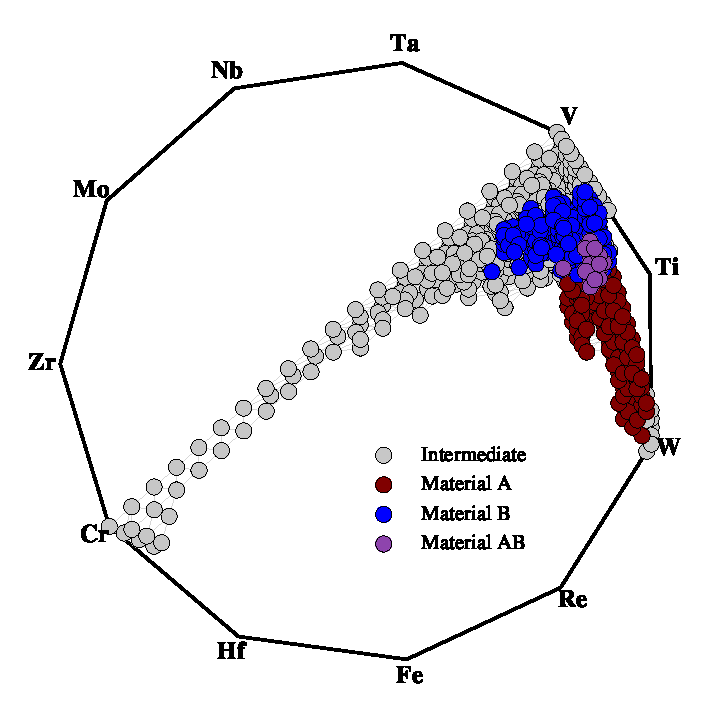
\includegraphics[width=0.75\linewidth]{figures/fig2_categories.pdf}
  \caption{Material classes of the \(686\) compositions of the design region
  (Subgraph~1), projected onto the eleven-element composition space: Material~A
  (plasma-facing, maroon), Material~B (structural, blue), Material~AB (both,
  purple), and Intermediate (neither, grey).}
  \label{fig:categories}
\end{figure}

The terminal alloys selected with \Cref{eq:ends} from the \(157\) plasma-facing (A
or AB) and \(187\) structural (B or AB) candidates are \ch{W90V5Re5}, with the
highest solidus (\(3449\)~K) and a yield strength of \(310\)~MPa at
\(600^{\circ}\)C, and \ch{W15V75Ti10}, with the highest Pugh ratio (\(3.03\)) and a
yield strength of \(285\)~MPa at \(650^{\circ}\)C. Neither terminal is a pure
element: the class definitions alone move both ends of the wall into
multicomponent alloys. Their linear CTE at \(600^{\circ}\)C, \(5.03\) and
\(9.28\times10^{-6}\)~K\(^{-1}\), sets the expansion change of
\(4.2\times10^{-6}\)~K\(^{-1}\) that the gradient must accommodate.


\subsection{Gradient Path with Monotonic CTE and Solidus}
\label{subsec:path}

A gradient that joins the two materials while satisfying every requirement exists,
and it is as short as any gradient between these terminals can be. Of the \(686\)
compositions of the design region, \(293\) are admissible layers
(\Cref{eq:admissible}), and of the \(7{,}348\) directed single-exchange steps,
\(2{,}714\) join two admissible layers and satisfy \Cref{eq:monotone}. Dijkstra's
algorithm on this graph returned a path of \(16\) steps (\(17\) alloys) from
\ch{W90V5Re5} to \ch{W15V75Ti10} (Fig.~\ref{fig:path-map}, Table~\ref{tab:path}),
verified step by step, with \(\mathrm{LOM}=0\). No path between these terminals can
be shorter, with or without monotonicity: \(75\)~at.\% W and \(5\)~at.\% Re must be
removed, \(5\)~at.\% per step. Requiring the CTE and the solidus to be monotonic at
the same time therefore adds no layers to the wall. Several paths share this
minimum length; they are equally optimal, and Dijkstra's algorithm returns one of
them deterministically.

\begin{figure}[H]
  \centering
  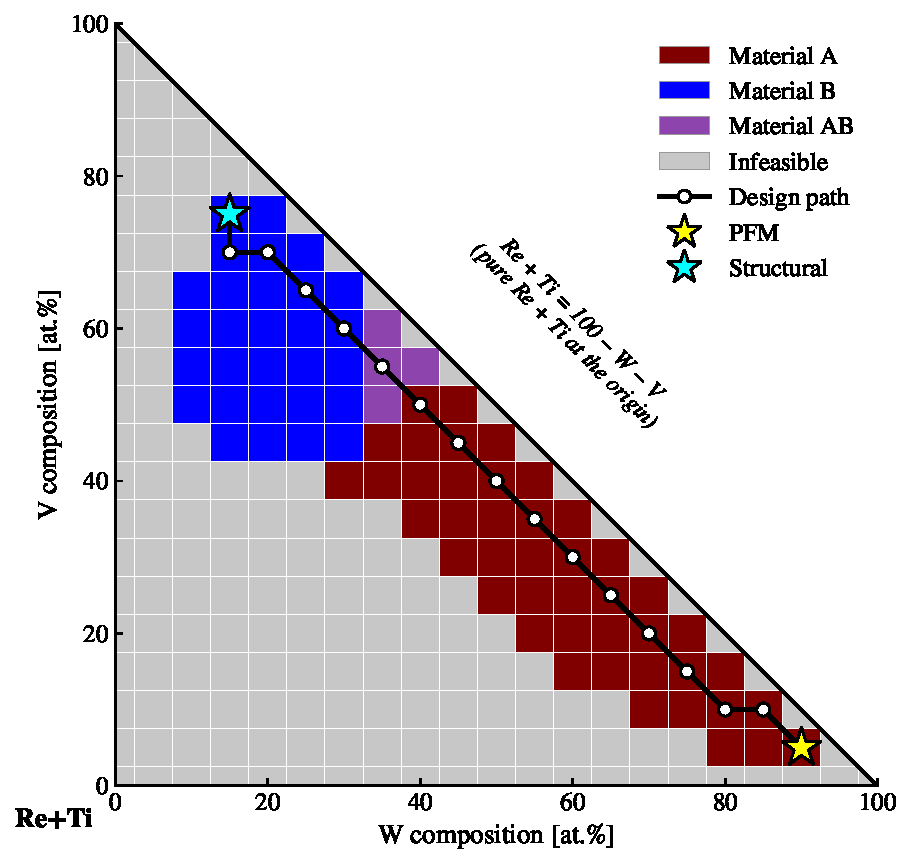
\includegraphics[width=\linewidth]{figures/fig3_design_path_map.pdf}
  \caption{The design path in W--V composition space, with the remaining path
  elements (Ti and Re) as the balance, so that the origin corresponds to pure
  Ti\(+\)Re. Each cell of the \(5\)~at.\% grid is coloured by its material class if
  it is an admissible path layer (Material~A, maroon; B, blue; AB, purple) and grey
  if any screen removes it. The path (black line, one marker per layer) runs from the
  plasma-facing terminal \ch{W90V5Re5} (yellow star) to the structural terminal
  \ch{W15V75Ti10} (cyan star).}
  \label{fig:path-map}
\end{figure}

The path divides the expansion change of the wall into sixteen small, same-signed
steps (Fig.~\ref{fig:path-profiles}). The linear CTE rises at every step, from
\(5.03\) to \(9.28\times10^{-6}\)~K\(^{-1}\) at \(600^{\circ}\)C and from \(5.06\) to
\(9.36\times10^{-6}\)~K\(^{-1}\) at \(650^{\circ}\)C, in nearly equal increments of
\(0.19\)--\(0.28\times10^{-6}\)~K\(^{-1}\). The largest step is less than a
twenty-fifth of the mismatch of about \(8\times10^{-6}\)~K\(^{-1}\) at a direct
tungsten--steel joint~\cite{fgmWsteelCGS2022}. The solidus falls at every step, from
\(3449\) to \(2262\)~K, most steeply (\(150\)--\(160\)~K per step) in the first two
tungsten-rich layers, so every layer melts at a temperature at least as high as the
layers behind it, matching the temperature drop through the wall.

\begin{figure}[H]
  \centering
  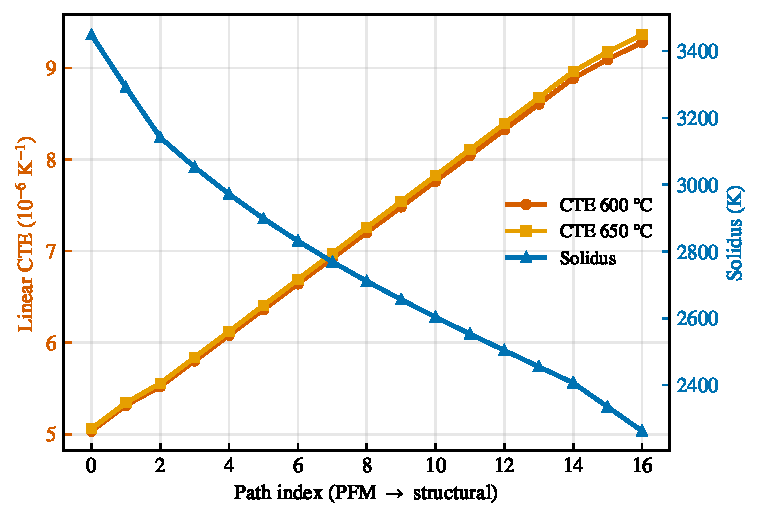
\includegraphics[width=\linewidth]{figures/fig4_cte_solidus_along_path.pdf}
  \caption{Linear CTE at \(600\) and \(650^{\circ}\)C (left axis, vermillion and
  orange) and solidus (right axis, blue) along the design path, from the plasma-facing
  terminal (path index~0) to the structural terminal (path index~16). The CTE never
  decreases and the solidus never increases from one layer to the next.}
  \label{fig:path-profiles}
\end{figure}

Properties that were not constrained along the path follow the same two-material
logic. The Pugh ratio rises from \(2.00\) to \(3.03\) without a single decrease, so
ductility increases toward the load-bearing side, because every step removes
tungsten or adds vanadium or titanium. The yield strength exceeds the EUROFER97-level
limits on every layer, with minima of \(307\)~MPa at \(600^{\circ}\)C and
\(285\)~MPa at \(650^{\circ}\)C at the two terminals and a maximum of \(824\)~MPa at
\(600^{\circ}\)C for \ch{W55V35Ti5Re5}, where W and V are most mixed, so the graded
layers are stronger than either material they join. The path passes through the
classes in order, eleven Material~A layers, two Material~AB layers, and four
Material~B layers (Table~\ref{tab:path}).

\begin{table*}[!t]
\centering
\caption{The design path: seventeen alloys connected by sixteen single
\(5\)~at.\% exchanges, from the plasma-facing terminal (layer~0) to the structural
terminal (layer~16). The linear CTE is non-decreasing at both temperatures and the solidus
non-increasing at every step; the Pugh ratio and yield strength are reported, not
constrained.}
\label{tab:path}
\begin{tabular}{cllcccccc}
\toprule
Layer & Composition (at.\%) & Step & \(T_s\) (K) & \(\alpha_{600}\) & \(\alpha_{650}\) & \(B/G\) & \(\sigma_y^{600}\) / \(\sigma_y^{650}\) (MPa) & Class \\
 & & & & \multicolumn{2}{c}{(\(10^{-6}\)~K\(^{-1}\))} & & & \\
\midrule
0  & W$_{90}$V$_{5}$Re$_{5}$         & --                  & 3449 & 5.03 & 5.06 & 2.00 & 310 / 294 & A \\
1  & W$_{85}$V$_{10}$Re$_{5}$        & W\,$-5$, V\,$+5$    & 3292 & 5.31 & 5.34 & 2.05 & 505 / 483 & A \\
2  & W$_{80}$V$_{10}$Ti$_{5}$Re$_{5}$ & W\,$-5$, Ti\,$+5$  & 3141 & 5.52 & 5.56 & 2.07 & 506 / 483 & A \\
3  & W$_{75}$V$_{15}$Ti$_{5}$Re$_{5}$ & W\,$-5$, V\,$+5$   & 3052 & 5.80 & 5.84 & 2.12 & 639 / 612 & A \\
4  & W$_{70}$V$_{20}$Ti$_{5}$Re$_{5}$ & W\,$-5$, V\,$+5$   & 2972 & 6.08 & 6.12 & 2.18 & 732 / 702 & A \\
5  & W$_{65}$V$_{25}$Ti$_{5}$Re$_{5}$ & W\,$-5$, V\,$+5$   & 2898 & 6.36 & 6.41 & 2.24 & 791 / 758 & A \\
6  & W$_{60}$V$_{30}$Ti$_{5}$Re$_{5}$ & W\,$-5$, V\,$+5$   & 2831 & 6.64 & 6.69 & 2.30 & 820 / 786 & A \\
7  & W$_{55}$V$_{35}$Ti$_{5}$Re$_{5}$ & W\,$-5$, V\,$+5$   & 2769 & 6.92 & 6.97 & 2.36 & 824 / 789 & A \\
8  & W$_{50}$V$_{40}$Ti$_{5}$Re$_{5}$ & W\,$-5$, V\,$+5$   & 2711 & 7.20 & 7.26 & 2.43 & 804 / 769 & A \\
9  & W$_{45}$V$_{45}$Ti$_{5}$Re$_{5}$ & W\,$-5$, V\,$+5$   & 2656 & 7.48 & 7.54 & 2.50 & 765 / 730 & A \\
10 & W$_{40}$V$_{50}$Ti$_{5}$Re$_{5}$ & W\,$-5$, V\,$+5$   & 2603 & 7.76 & 7.83 & 2.57 & 709 / 675 & A \\
11 & W$_{35}$V$_{55}$Ti$_{5}$Re$_{5}$ & W\,$-5$, V\,$+5$   & 2553 & 8.04 & 8.11 & 2.65 & 638 / 606 & AB \\
12 & W$_{30}$V$_{60}$Ti$_{5}$Re$_{5}$ & W\,$-5$, V\,$+5$   & 2503 & 8.32 & 8.39 & 2.73 & 557 / 526 & AB \\
13 & W$_{25}$V$_{65}$Ti$_{5}$Re$_{5}$ & W\,$-5$, V\,$+5$   & 2455 & 8.60 & 8.68 & 2.82 & 467 / 439 & B \\
14 & W$_{20}$V$_{70}$Ti$_{5}$Re$_{5}$ & W\,$-5$, V\,$+5$   & 2406 & 8.89 & 8.96 & 2.91 & 373 / 349 & B \\
15 & W$_{15}$V$_{70}$Ti$_{10}$Re$_{5}$ & W\,$-5$, Ti\,$+5$ & 2334 & 9.09 & 9.17 & 2.96 & 342 / 319 & B \\
16 & W$_{15}$V$_{75}$Ti$_{10}$        & Re\,$-5$, V\,$+5$  & 2262 & 9.28 & 9.36 & 3.03 & 307 / 285 & B \\
\bottomrule
\end{tabular}
\end{table*}

The path is also simple to build (Fig.~\ref{fig:path-composition}). Although it was
planned in an eleven-element space, it uses only W, V, Ti, and Re: tungsten falls
from \(90\) to \(15\)~at.\% as vanadium rises from \(5\) to \(75\)~at.\%, titanium
enters at \(5\)~at.\% in the second step and rises to \(10\)~at.\% near the
structural end, and rhenium stays at \(5\)~at.\% until the final step. The gradient
can thus be deposited mainly by varying the W and V feeds, with the Ti and Re
additions changed only three times. Iron is absent from every layer, so the
tungsten--iron intermetallics that limit conventional tungsten-to-steel gradients
cannot form anywhere along the wall.

\begin{figure}[H]
  \centering
  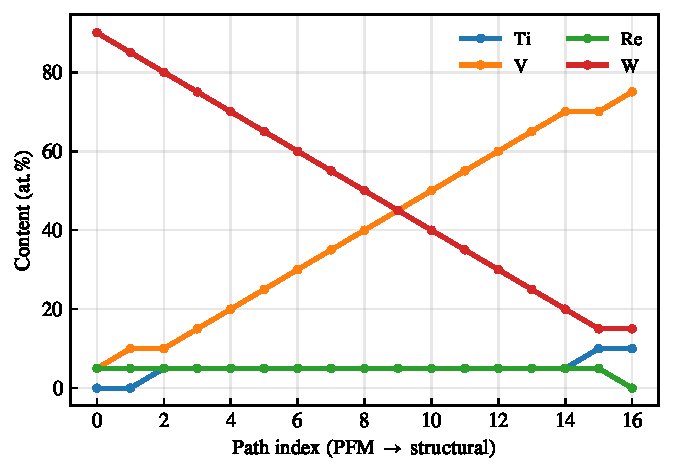
\includegraphics[width=0.9\linewidth]{figures/fig5_composition_profile.pdf}
  \caption{Composition of W, V, Ti, and Re along the design path, from the
  plasma-facing terminal (path index~0) to the structural terminal (path
  index~16). Each step exchanges \(5\)~at.\% of one element for another: a W--V
  gradient with Ti added at layers~2 and~15 and Re removed at the final layer.}
  \label{fig:path-composition}
\end{figure}

Together, these results show that the two materials of the first wall can be joined
by a single-phase, reduced-activation gradient in which every requirement holds
layer by layer, and that the two monotonicity requirements cost nothing in the
number of layers. Two limitations apply. First, the properties are model estimates,
the yield strength from the Maresca--Curtin model, the Pugh ratio from a rule of
mixtures, and the solidus and CTE from CALPHAD; they are suited to ranking
compositions and setting the direction of the gradient, but the values along the
path, in particular for the vanadium-rich layers, should be confirmed by measurement
on the terminal alloys and selected intermediate layers before the gradient is
built. Second, the path ensures that the CTE changes in one direction only, but the
thermal stresses in the graded wall were not computed; such an analysis requires
the layer thicknesses and the through-wall temperature field and was considered
outside the scope of this work, as it would not change the path design methodology.

\section{Conclusions and Future Work}
\label{sec:conclusion}

The joint between the plasma-facing and structural materials of the fusion first wall
is limited by thermal-expansion mismatch and by the formation of brittle W--Fe
intermetallics. In this work, a compositionally graded alloy was designed to bridge
the two sides within an eleven-element refractory composition space. Activation
screening was performed by linear programming on the composition-linear FLARE model,
CALPHAD calculations were used to restrict the space to single-phase BCC compositions
of adequate thermal conductivity, and the compositions of the resulting design region
were classified as plasma-facing or structural materials by solidus, Pugh ratio, and
EUROFER97-level yield strength. The gradient path between the two terminal alloys was
planned on the composition graph with the lack-of-monotonicity cost function of Kirk
et al., with monotonic CTE and solidus imposed as hard constraints. The primary
conclusions that can be drawn from this work are as follows:

\begin{enumerate}
\item Of the \(61{,}303\) unique activation-feasible compositions, \(700\) are
single-phase BCC and thermally conductive, and \(686\) of these form one connected
design region. Phase stability is by far the most restrictive of the property
criteria.
\item Imposing monotonicity as hard constraints reduces the cost function to path
length, so the optimal path is found exactly by Dijkstra's algorithm, with no
penalty weight to select.
\item The resulting path joins \ch{W90V5Re5} to \ch{W15V75Ti10} in sixteen single
\(5\)~at.\% exchanges, the minimum possible for these terminals, so the monotonicity
constraints are met at no cost in path length.
\item Along the path, the linear CTE at \(600^{\circ}\)C rises from \(5.03\) to
\(9.28\times10^{-6}\)~K\(^{-1}\) in increments of at most
\(0.28\times10^{-6}\)~K\(^{-1}\), the solidus falls from \(3449\) to \(2262\)~K, and
every layer remains single-phase BCC, reduced in activation, and at least as strong as
EUROFER97 at \(600\) and \(650^{\circ}\)C. The Pugh ratio, although not constrained,
also rises at every step, from \(2.00\) to \(3.03\).
\item Despite being planned in an eleven-element space, the path contains only four
elements, a W--V gradient with small Ti and Re additions, which simplifies its
deposition.
\end{enumerate}

The formulation generalizes in both of its parts. The constraint-first screening
applies to any model whose responses are linear in composition, and the path design
applies to any graded alloy that must be monotonic in one or more properties. For
future work in this area, a number of steps could be taken. The CTE, solidus, and
strength of the terminal alloys and selected intermediate layers should be measured
to validate the model estimates. The gradient should then be fabricated by additive
manufacturing and its microstructure characterized along the build. Finally, the
thermal stresses and thermomechanical response of the graded wall under first-wall
heat loads should be evaluated.
% An edge-localized-mode assessment independently validates the design,
% with the plasma-facing terminal carrying a melting margin of \(+1650\)~K and
% the margin remaining positive along the gradient precisely through its
% plasma-facing extent, the structural layers behind it sitting shielded from
% surface loading.

\input{05_code-availability}
\input{06_ai-decleration}
\input{07_competing-interest-decleration}
\input{08_acknowledgments}
\input{09_CRediT}

\bibliographystyle{elsarticle-num}
\bibliography{ref}

\end{document}
